\documentclass[12pt,a4paper]{article}

\usepackage[utf8]{inputenc}
\usepackage[T1]{fontenc}
\usepackage{polski}
\usepackage{amsmath}
\usepackage{pgfplots}
\usepackage{tikz}
\usepackage{lmodern}	%fancy font
\usepackage{textcomp}
\usepackage{indentfirst}
\usepackage{graphicx}
\usepackage{caption}
\usepackage{subcaption}
\usepackage{here}
\usepackage{tabto}
\usepackage{multicol}

\setlength{\textheight}{24cm}
\setlength{\textwidth}{15.92cm}
\setlength{\footskip}{10mm}
\setlength{\oddsidemargin}{0mm}
\setlength{\evensidemargin}{0mm}
\setlength{\topmargin}{0mm}
\setlength{\headsep}{5mm}


\begin{document}

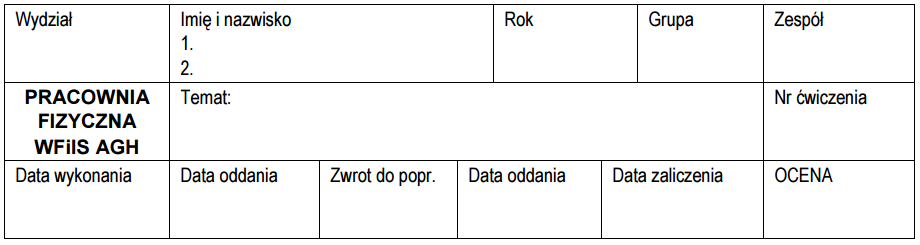
\includegraphics[scale=0.6]{img_fiz/header_table}

\section{Cel ćwiczenia}

Zapoznanie się z działaniem ogniwa słonecznego i wyznaczenie:

\begin{itemize}
\item charakterystyk prądowo-napięciowych dla różnych rodzajów ogniw
przy ustalonym oświetleniu
\item Zależności gęstości prądu ogniwa jako funkcji napięcia na sekcję
\item Sprawności badanych ogniw
\end{itemize}



\section{Przebieg ćwiczenia}

\subsection{Układ doświadczalny}
Skonstruowano obwód z rys.1a i układ jak na rys. 1b.

\begin{figure}[H]
\centering
\begin{subfigure}{.5\textwidth}
  \centering
  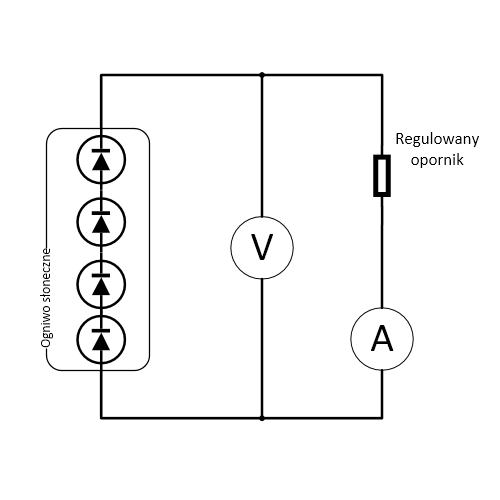
\includegraphics[width=1\textwidth]{img_fiz/Circuit}
  \caption{Obwód z ogniwem}
  \label{fig:sub1}
\end{subfigure}%
\begin{subfigure}{.5\textwidth}
  \centering
  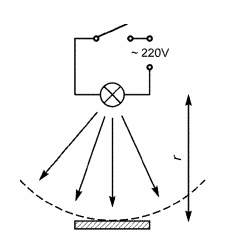
\includegraphics[width=1\textwidth]{img_fiz/Lamp}
  \caption{Lampa i ogniwo słoneczne}
  \label{fig:sub2}
\end{subfigure}
\caption{Układ doświadczalny}
\label{fig:test}
\end{figure}


\subsection{Wyniki pomiarów}

\begin{table}[H]
\centering
\caption{Natężenie światła}
\label{my-label}
\begin{tabular}{|p{3cm}|p{3cm}|}
\hline
$\phi$ {[}$W/m^2${]}	& $\phi$ śr. {[}$W/m^2${]}\\
\hline
60,0(3,6)				& 58,9(3,5)	\\
65,2(3,8)				&			\\
54,5(3,3)				&			\\
55,8(3,4)				&			\\
\hline   
\end{tabular}
\end{table}

\begin{table}[H]
\centering
\caption{Ogniwo polikrystaliczne - stałe}
\label{polistale}
\begin{tabular}{|p{2cm}|p{2cm}|p{2cm}|}
\hline
N & S {[}$cm^2${]} & N*S {[}$cm^2${]}   \\
\hline
8 & 7,8(1) & 62,4(1) \\
\hline
\end{tabular}
\end{table}

\begin{table}[H]
\centering
\caption{Ogniwo polikrystaliczne - pomiary}
\label{poliwyniki}
\begin{tabular}{|p{2cm}|p{2cm}|p{2cm}|p{2cm}|p{2cm}|}
\hline
I {[}$mA${]}	& U {[}$V${]}	& P  {[}$mW${]}	& U/N {[}$V${]}	& I/S {[}$A/m^2${]} \\
\hline
0,1243(18)		& 2,63(8)		& 0,33(1)		& 0,33(1)		& 0,159(3)\\
0,1694(23)		& 2,62(8)		& 0,44(2)		& 0,33(1)		& 0,217(4)\\
0,20(6)			& 2,61(8)		& 0,52(16)		& 0,33(1)		& 0,26(8)\\
0,60(6)			& 2,53(8)		& 1,52(17)		& 0,32(1)		& 0,77(8)\\
1,00(7)			& 2,46(8)		& 2,46(19)		& 0,31(1)		& 1,28(9)\\
1,43(7)			& 2,37(8)		& 3,39(21)		& 0,30(1)		& 1,83(10)\\
1,63(7)			& 2,33(8)		& 3,80(22)		& 0,29(1)		& 2,09(10)\\
1,85(8)			& 2,28(8)		& 4,22(23)		& 0,29(1)		& 2,37(10)\\
2,00(8)			& 2,25(8)		& 4,50(24)		& 0,28(1)		& 2,56(10)\\
2,24(8)			& 2,18(8)		& 4,88(25)		& 0,27(1)		& 2,87(11)\\
2,43(8)			& 2,12(8)		& 5,15(26)		& 0,27(1)		& 3,12(11)\\
2,69(8)			& 2,05(8)		& 5,51(27)		& 0,26(1)		& 3,45(12)\\
2,99(9)			& 1,966(25)		& 5,88(19)		& 0,246(3)		& 3,83(12)\\
3,22(9)			& 1,892(25)		& 6,09(19)		& 0,237(3)		& 4,13(13)\\
3,37(9)			& 1,89(8)		& 6,37(31)		& 0,24(1)		& 4,32(13)\\
3,55(9)			& 1,735(23)		& 6,16(18)		& 0,217(3)		& 4,55(13)\\
3,59(9)			& 1,80(8)		& 6,46(32)		& 0,23(1)		& 4,60(13)\\
3,87(10)		& 1,515(21)		& 5,86(17)		& 0,189(3)		& 4,96(14)\\
4,07(10)		& 1,329(19)		& 5,41(15)		& 0,166(2)		& 5,22(14)\\
4,25(10)		& 1,109(17)		& 4,71(13)		& 0,139(2)		& 5,45(15)\\
4,41(10)		& 0,793(14)		& 3,50(10)		& 0,099(2)		& 5,65(15)\\
4,51(10)		& 0,671(12)		& 3,03(9)		& 0,084(2)		& 5,78(15)\\
4,69(10)		& 0,530(11)		& 2,49(8)		& 0,066(1)		& 6,01(15)\\
\hline
\end{tabular}
\end{table}

\newpage

\begin{table}[H]
\centering
\caption{Ogniwo monokrystaliczne - stałe}
\label{monostale}
\begin{tabular}{|p{2cm}|p{2cm}|p{2cm}|}
\hline
N & S {[}$cm^2${]} & N*S {[}$cm^2${]}   \\
\hline
1 & 63,0(1) & 63,0(1) \\
\hline
\end{tabular}
\end{table}

\begin{table}[H]
\centering
\caption{Ogniwo monokrystaliczne - pomiary}
\label{mono}
\begin{tabular}{|p{2cm}|p{2cm}|p{2cm}|p{2cm}|p{2cm}|}
\hline
I {[}$mA${]}	& U {[}$V${]}	& P  {[}$mW${]}	& U/N {[}$V${]} & I/S {[}$A/m^2${]} \\ 
\hline
0,6(6)			& 0,46(1)		& 0,27(27)		& 0,46(1)		& 0,10(9)\\
1,0(6)			& 0,46(1)		& 0,46(27)		& 0,46(1)		& 0,16(9)\\
1,7(6)			& 0,46(1)		& 0,78(27)		& 0,46(1)		& 0,27(9)\\
2,2(6)			& 0,46(1)		& 1,01(27)		& 0,46(1)		& 0,35(10)\\
3,6(6)			& 0,46(1)		& 1,64(28)		& 0,46(1)		& 0,57(10)\\
5,2(6)			& 0,45(1)		& 2,36(29)		& 0,45(1)		& 0,83(10)\\
7,1(6)			& 0,45(1)		& 3,21(30)		& 0,45(1)		& 1,13(10)\\
10,6(7)			& 0,45(1)		& 4,76(33)		& 0,45(1)		& 1,68(11)\\
15,7(7)			& 0,44(1)		& 6,96(36)		& 0,44(1)		& 2,49(12)\\
\hline
\end{tabular}
\end{table}


\begin{center}
\begin{tikzpicture}[scale=1.5]
\begin{axis}[
    title={Zależność gęstości prądu od napięcia na sekcję},
    xlabel={Napięcie na sekcję U/N [V]},
    ylabel={Gęstość prądu j [$A/m^2$]},
    xmin=0, xmax=0.5,
    ymin=0, ymax=8,
    xtick={0,0.1,0.2,0.3,0.4, 0.5},
    ytick={0,1,2,3,4,5,6,7, 8, 9},
    legend image post style=only marks,
    legend pos=north east,
    grid=major,
    grid style=dashed,
]
 
\addplot+[
    color=blue,
    mark=x,
    draw=none,
    error bars/.cd,
    x dir=both,x explicit,
    y dir=both,y explicit,
    ]
    coordinates {
    (0.33,	0.159) +- (0.01,0.003)
	(0.33,	0.217) +- (0.01,0.004)
	(0.33,	0.26) +- (0.01,0.08)
	(0.32,	0.77) +- (0.01,0.08)
	(0.31,	1.28) +- (0.01,0.09)
	(0.30,	1.83) +- (0.01,0.10)
	(0.29,	2.09) +- (0.01,0.10)
	(0.29,	2.37) +- (0.01,0.10)
	(0.28,	2.56) +- (0.01,0.10)
	(0.27,	2.87) +- (0.01,0.11)
	(0.27,	3.12) +- (0.01,0.11)
	(0.26,	3.45) +- (0.01,0.12)
	(0.246,	3.83) +- (0.003,0.12)
	(0.237,	4.13) +- (0.003,0.13)
	(0.24,	4.32) +- (0.01,0.13)	
	(0.217,	4.55) +- (0.003,0.13)
	(0.23,	4.60) +- (0.01,0.13)
	(0.189,	4.96) +- (0.003,0.14)
	(0.166,	5.22) +- (0.002,0.14)
	(0.139,	5.45) +- (0.002,0.15)
	(0.099,	5.65) +- (0.002,0.15)
	(0.084,	5.78) +- (0.002,0.15)
	(0.066,	6.01) +- (0.001,0.15)
    };
    \addlegendentry{Polikrystaliczne}
    
    \addplot+[
    color=red,
    mark=x,
    draw=none,
    error bars/.cd,
    x dir=both,x explicit,
    y dir=both,y explicit,
    ]
    coordinates {
    (0.46, 0.10) +- (0.01,0.09)
	(0.46, 0.16) +- (0.01,0.09)
	(0.46, 0.27) +- (0.01,0.09)
	(0.46, 0.35) +- (0.01,0.10)
	(0.46, 0.57) +- (0.01,0.10)
	(0.45, 0.83) +- (0.01,0.10)
	(0.45, 1.13) +- (0.01,0.10)
	(0.45, 1.68) +- (0.01,0.11)
	(0.44, 2.49) +- (0.01,0.12)
    };
    \addlegendentry{Monokrystaliczne}
 
\end{axis}
\end{tikzpicture}
\end{center}

\newpage

\subsection{Omówienie wyników}
Pomiar napięcia i natężenia dla ogniwa polikrystalicznego dał o wiele ciekawszą krzywą, mówiącą więcej o ogólnym kształcie funkcji niż dla ogniwa monokrystalicznego, gdyż zakres oporu jakim dysponowaliśmy nie pozwolił na znaczne zmiany napięcia na tym ogniwie (różnica 0,02 V między napięciami na najmniejszym a największym możliwym oporze). Dlatego też choć maksymalna moc dla obu ogniw jest podobna, około 7 mW, można podejrzewać, że maksimum mocy dla ogniwa monokrystalicznego można zaobserwować dla oporu mniejszego niż najmniejszy dostępny przy oporniku, którym dysponowaliśmy. \\
W punkcie największej zmierzonej mocy ogniwo monokrystaliczne ma większe napięcie na sekcję, zaś ogniwo polikrystaliczne ma większą gęstość prądu.\\\\
Sprawność ogniwa wynosi:
$\eta = \dfrac{P}{P_{\text{źródła}}} = \dfrac{P}{\phi \times S}$ \\
zatem dla ogniwa:\\
\begin{itemize}
\item polikrystalicznego:
$\eta = \dfrac{6,46 \times 10^{-3} W}{58,9 \frac{W}{m^2} \times 62,4 \times 10^{-4} m^2} \approx 1,76(14) \%$ \\\\
\item monokrystalicznego:
$\eta = \dfrac{6,96 \times 10^{-3} W}{58,9 \frac{W}{m^2} \times 62,4 \times 10^{-4} m^2} \approx 1,88(15) \% $
\end{itemize}
Tak niska sprawność może wynikać np. z faktu, że ogniwo jest już stare i zużyte, może mieć też zanieczyszczoną powierzchnię, ponadto światło lampy mogło mieć niewłaściwą długość fali, przez co efekt fotowoltaiczny nie był odpowiednio wydajny.

\subsection{Dyskusja niepewności i błędów}
Na używanych elektronicznych przyrządach pomiarowych nie naniesiono informacji o ich dokładności, dlatego niepewności oszacowano na podstawie obserwacji działania przyrządów w trakcie wykonywania pomiarów (np. porównanie zbliżonych wartości pomiaru na różnych zakresach) i typowych charakterystyk przyrządów pomiarowych danego typu.\\
Niepewności pomiaru napięcia oraz natężenia prądu, a także natężenia światła obliczono zgodnie z wzorem:
$$u(x) = \frac{\Delta x}{\sqrt{3}},\ \Delta x = C_1 \times x + C_2 \times r^x
\text{, gdzie: $C_1, C_2$ - stałe przyrządu, $r^x$ - zakres miernika}$$

Zakresy mierników podane są w arkuszu z wynikami pomiarów, natomiast stałe $C_1$ oraz $C_2$ dobrano jak następuje:
\begin{itemize}
\TabPositions{3cm}
\item amperomierz:\tab$C_1^I = 1\%$, $C_2^I = 0,5\%$
\item woltomierz:\tab$C_1^U = 1\%$, $C_2^U = 0,5\%$
\item luksomierz:\tab$C_1^\phi = 5\%$, $C_2^\phi = 0,5\%$
\end{itemize}

Ostateczna wartość natężenia światła $\phi$ jest średnią z czterech pomiarów, jednak każdy z nich został wykonany przy innym boku ogniwa, dlatego nie potraktowano ich jako serii statystycznej jednej wielkości, lecz zastosowano oszacowanie niepewności typu B do uzyskanej wartości średniej, tak jakby to ona była wynikiem pomiaru.

Całkowita powierzchnia ogniwa $S$ była dana na płytce z ogniwem bez informacji o dokładności, zatem za jej niepewność przyjęto ostatnią podaną cyfrę.

Niepewności obliczono według następujących wzorów:\\
$$u(I) = \frac{1}{\sqrt{3}} (C_1^I \times I + C_2^I \times r^I)$$
$$u(U) = \frac{1}{\sqrt{3}} (C_1^U \times U + C_2^U \times r^U)$$
$$u(\phi) = \frac{1}{\sqrt{3}} (C_1^\phi \times \phi + C_2^\phi \times r^\phi)$$
$$u_c(P) = u_c(U \times I) = \sqrt{(I \times u(U))^2 + (U \times u(I))^2}$$
$$u(U/N) = u(U)/N$$
$$u_c(I/S) = \sqrt{((1/S) \times u(I))^2 + ((I/S^2) \times u(S))^2}$$
$u_c(\eta) = u_c(P/(\phi \times S))\\ \text{\qquad\ } = \sqrt{((1/(\phi \times S) \times u_c(P))^2 + (P/(\phi^2 \times S) \times u(\phi))^2 + (P/(\phi \times S^2) \times u(S))^2}$\\

Należy odnotować, że opornik na płytce z ogniwem monokrystalicznym był rozstrojony, tzn. przy kręceniu jego gałką regulującą, rezystancja rosła zgodnie z oczekiwaniami, w pewnym momencie gwałtownie malała, a potem znów gwałtownie rosła, by powrócić do poziomu sprzed spadku. Z tego powodu część wyników pomiaru odrzucono jako nieweryfikowalne bez użycia innego opornika. Również dlatego zakres amperomierza użyty przy pomiarach na ogniwie monokrystalicznym jest nieadekwatny w stosunku do nieodrzuconej części zmierzonych natężeń, przez co ich niepewności są stosunkowo duże.

\end{document}
